\documentclass[a4paper,12pt,pdftex]{scrartcl}

\usepackage[american]{babel}
\usepackage[utf8]{inputenc}

\usepackage{listings}
\lstset{
  basicstyle=\ttfamily \scriptsize,
  showstringspaces=false
}
\lstset{xleftmargin=0cm}
\lstset{language=bash}
\lstset{frame=single}

\lstset{breaklines=true}

\usepackage{graphicx}
%\usepackage{cmbright}   

\parindent0cm
\parskip2.5mm

\title{PIOSim MPIwrapper}
\author{Paul Müller}

\begin{document}

\maketitle

\begin{abstract}
  The MPI wrapper is a static library that can be used to log MPI
  function calls which occur during the execution of a program. The
  log files are intended to be used by the PIOsimHD simulator project.

  This document describes the use, internal structure and extension
  possibilities of the MPI wrapper.
\end{abstract}

\tableofcontents

\section{Using the wrapper}

\subsection{Requirements}

The MPI wrapper project references the HDTraceWritingCLibrary
project. It must be built before building the MPI wrapper:
\begin{lstlisting}
cd PIOsimHD/HDTraceWritingCLibrary/
make
\end{lstlisting}

\verb/libglib/ is also needed.

\subsection{Building the wrapper}

The MPI wrapper library can be built either for the mpich or openmpi
implementation of MPI. Due to differences between the implementations
you cannot use one version of the wrapper for both.

To build the library for mpich, call make:
\begin{lstlisting}
cd PIOsimHD/PIOsimHD-Maint/mpiwrapperNew/
make
\end{lstlisting}

To build the library for openmpi, set the environment variable
\lstinline|MPIIMP=openmpi|:
\begin{lstlisting}
cd PIOsimHD/PIOsimHD-Maint/mpiwrapperNew/
MPIIMP=openmpi make
\end{lstlisting}

\subsection{Building the tests}
The directory
\lstinline|PIOsimHD/PIOsimHD-Maint/mpiwrapperNew/test/HDTests|
contains a number of programs to test the functionality of the
wrapper. These tests can be build via
\begin{lstlisting}
cd PIOsimHD/PIOsimHD-Maint/mpiwrapperNew/
make hdtest
\end{lstlisting}

\subsection{Example: Producing a trace}
In this example, the PIOsim project tree is located in the home
folder, and the necessary libraries have been built as described
above. I am going to compile and trace the \verb/mpi-io-test/ program
\cite{mpi-io-test}.
\begin{lstlisting}
cd $HOME
mkdir mpi-io-test
cd mpi-io-test/
wget http://mirror.anl.gov/pub/pvfs2/tests/mpi-io-test.c
mpicc -o mpi-io-test mpi-io-test.c \
 $HOME/PIOsimHD/PIOsimHD-Maint/mpiwrapperNew/libs/libHDTraceMPIWrapper.a \
 $HOME/PIOsimHD/HDTraceWritingCLibrary/lib/libhdTrace.a \
 `pkg-config --libs glib-2.0`
mpiexec -n 3 ./mpi-io-test
\end{lstlisting}  %$
Running the program will produce the following output

\begin{lstlisting}
# Using mpi-io calls.
nr_procs = 3, nr_iter = 1, blk_sz = 16777216, coll = 0
# total_size = 50331648
# Write: min_t = 1.177056, max_t = 1.613190, mean_t = 1.331647, var_t = 0.059641
# Read:  min_t = 0.448252, max_t = 0.544611, mean_t = 0.509273, var_t = 0.002816
Write bandwidth = 31.200076 Mbytes/sec
Read bandwidth = 92.417616 Mbytes/sec
D: [TRACER][node02.1.0] flushLog (hdTrace.c:955): flushing log length: 2172
D: [TRACER][node01.0.0] flushLog (hdTrace.c:955): flushing log length: 2130
D: [TRACER][node01.2.0] flushLog (hdTrace.c:955): flushing log length: 2172
\end{lstlisting}
This means everything went well and each of the three processes wrote
their own log files. The directory now contains three \verb/.trc/ and
three \verb/.info/ files. The latter need to be converted in order to
provide a format that is compatible with the simulator software and
other tools. The conversion is done via
\begin{lstlisting}
$HOME/PIOsimHD/PIOsimHD-Maint/mpiwrapperNew\
/scripts/project-description-merger.py \
  -o mpi-io-test.proj mpi-io-test_*.trc
\end{lstlisting} %$
The resulting four xml trace files can now be processed by other tools. 
The result of loading the files into HDJumpshot is shown in 
(\ref{fig:jumpshot-open}), (\ref{fig:jumpshot})
\begin{figure}[h]
  \centering
  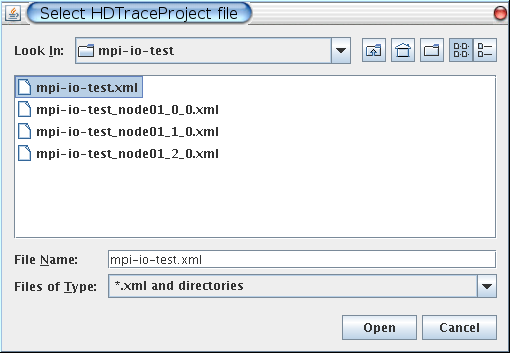
\includegraphics[scale=2]{img/jumpshot-open}
  \caption{Opening the project description file}
  \label{fig:jumpshot-open}
\end{figure}

\begin{figure}[h]
  \centering
  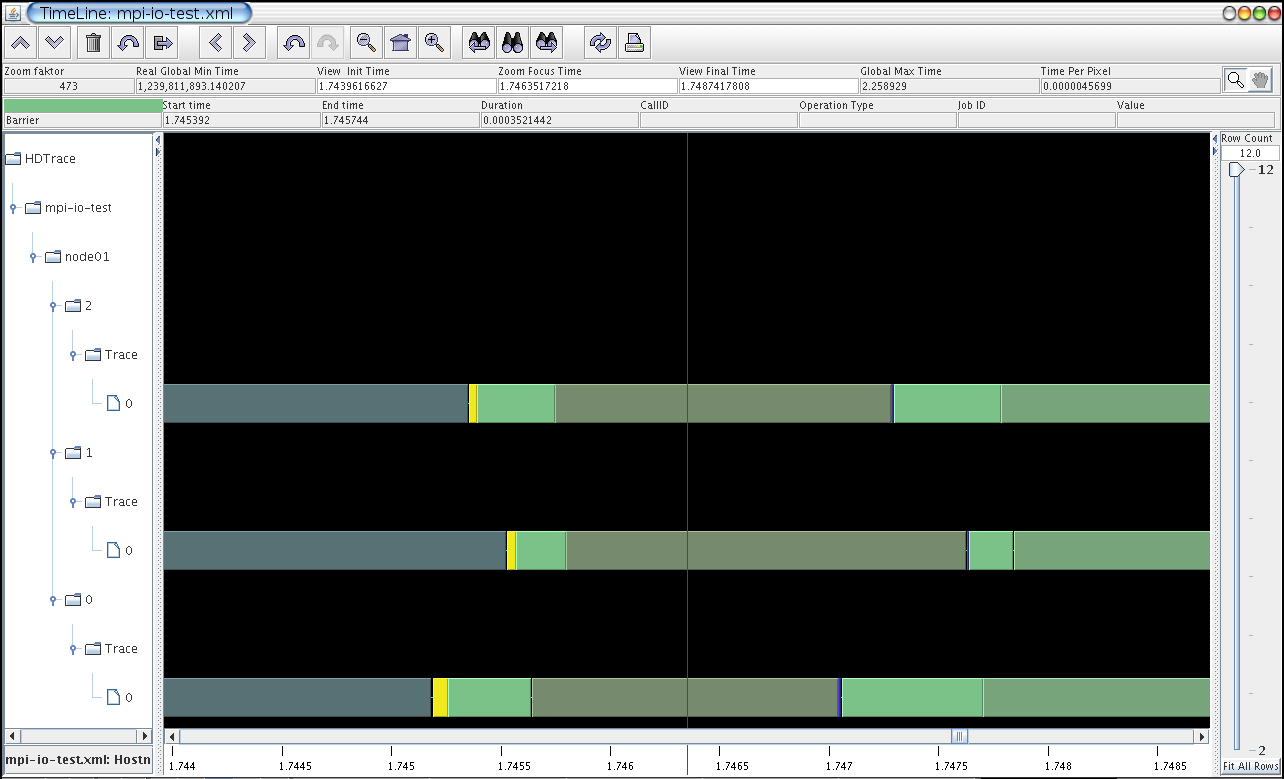
\includegraphics[scale=1]{img/jumpshot}
  \caption{mpi-io-test as displayed by Jumpshot}
  \label{fig:jumpshot}
\end{figure}


\section{Functionality}

\subsection{Goals}
The main goal of the MPI wrapper is to log the MPI interaction of a
parallel program. The log must contain the necessary information to
simulate the program at the MPI level and to meaningfully compare the
simulation results with the real program execution.  

When simulating the execution of traced programs, the simulator
assumes the program's logical execution to be independent of the
performance of individual MPI functions. It also assumes that the time
spent outside of the \emph{important} (i.e. communication and
input/output performing) functions does not depend on the performance
of those functions. Therefore it suffices to log every call of an
\emph{important} function combined with its start time (time of the
call), end time (time of the return) and the relevant function
arguments. Relevant arguments are those that indicate which ranks are
taking part in a communication, how much data is transferred and which
resources are being used.

The use of the following resources must be logged:
\begin{enumerate}
\item Files: Every file access via an MPI function must identify,
  which file is being accessed.
\item Communicators: The communicator indicates, which processes are
  taking part in a particular collective call and is needed to
  reconstruct, to which group an MPI call belongs to.
\item Types: Usually, transmission of data is performed on a number of
  instances of an MPI datatype. Because datatypes can contain holes
  and there are different strategies to transmit such complex
  datatypes, it is necessary to log the compositions of the datatypes
  that are used.
\item Requests: MPI allows the user to use nonblocking calls by
  returning an \verb MPI_Request  structure that can be used to poll the
  state of the call, or, for example, to use a blocking 
  \verb MPI_Wait . The latter is relevant for the simulation, because
  it halts the execution until the corresponding nonblocking call is
  finished, which must be simulated. 
\item Split collective function calls: There are also split collective
  function calls, that represent a nonblocking, collective access to a
  file. They are separated into a {\verb *_begin }  and an 
  {\verb *_end } routine, where the latter is equivalent to a 
  blocking wait. 
\end{enumerate}

There are two main kinds of data that should be logged: Data that
references only the local process such as the time and order of MPI
function calls, or the request structures that are used to keep track
of nonblocking function calls. The other kind has a global meaning,
such as files that are seen by all processes and communicators that
are created in collective calls and must be equal for all members of
the communicator. 

Logging of the process-local data can be done in a straightforward
fashion where each process writes to its own log file. There are
several possibilities to log the global data:
\begin{itemize}
\item Create a unique identifier for each global resource on its first
  use and communicate this identifier to all other processes. 
\item Create a process internal identifier and store, to which process
  it refers. Unify the different identifiers in a post-processing
  step.
\end{itemize}
Because it is our goal to disturb the program's behaviour as little as
possible we choose the second approach. Every process writes two
files, an \verb *.trc  and an \verb *.info  file. The latter holds the
mapping from process-identifiers to the actual global objects (files,
communicators). As a minor drawback, the trace must be processed by a
script to bring it in a simulator-compatible form. 

\subsubsection{Tracing method}
There are two main requirements that the wrapper library must fulfill:
\begin{itemize}
\item It must be easy usable with different MPI implementations, at least
  with Open MPI and MPICH
\item The use of the wrapper must be as easy as possible. 
\end{itemize}
For these reasons, the wrapper is implemented by creating an object
file that contains wrapper functions with the same name as the
important MPI functions. These functions perform the necessary logging
routines, pass the arguments to the underlying MPI library and pass
its return value back to the calling program. When the object file is
linked to a program, the wrapper functions hide the original MPI
functions. 

This is reasonably easy and the wrapper is mostly
independent of the used MPI implementation. (The \verb mpi.h  and 
\verb mpio.h  headers that are used to compile the MPI wrapper must be
the same that are used to compile the traced program.) Also, the
\verb/mpicc/ compiler can be used as usual.

One disadvantage of the approach is that we need to compile the
program that needs to be traced. That means we need to have its source
code (which is usually the case). Another problem could occur due to
an implementation detail of the wrapper: The wrapper functions need to
pass every call to the MPI library. This can easily be done because
the library provides every MPI function once using the \verb MPI_ and
once using the \verb/PMPI_/ prefix. Thus, passing the function call to
the MPI library is done by calling the corresponding PMPI
function. This means, the wrapper won't function correctly if the
program it is tracing makes use of the \verb/PMPI_/ names.

\subsection{Components}

\begin{figure}[t]
  \centering
  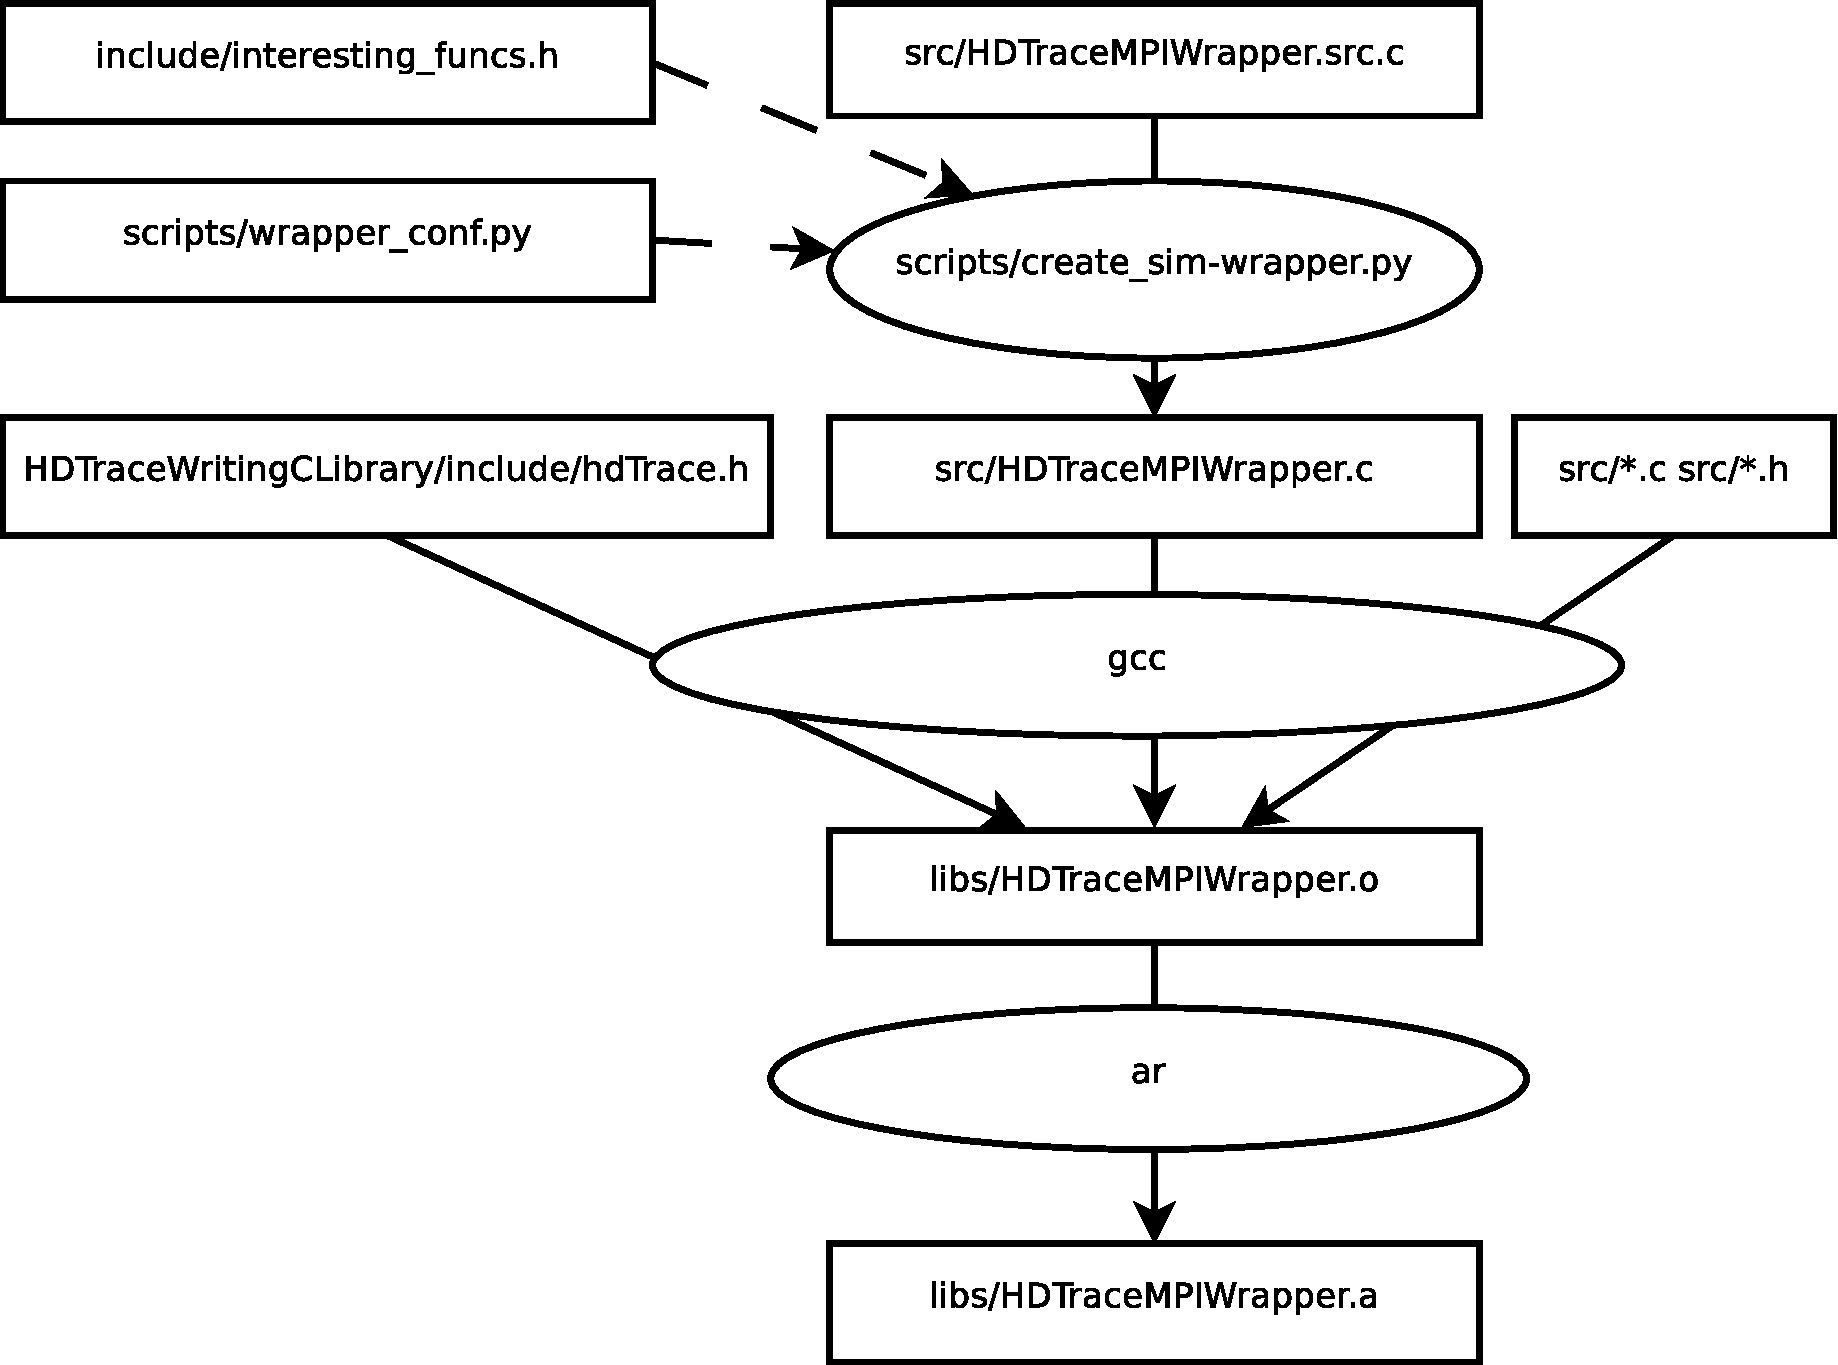
\includegraphics[width = 0.8 \textwidth]{img/building}
  \caption{Building the MPI wrapper library from source files.}
  \label{fig:building}
\end{figure}

\begin{figure}[h]
  \centering
  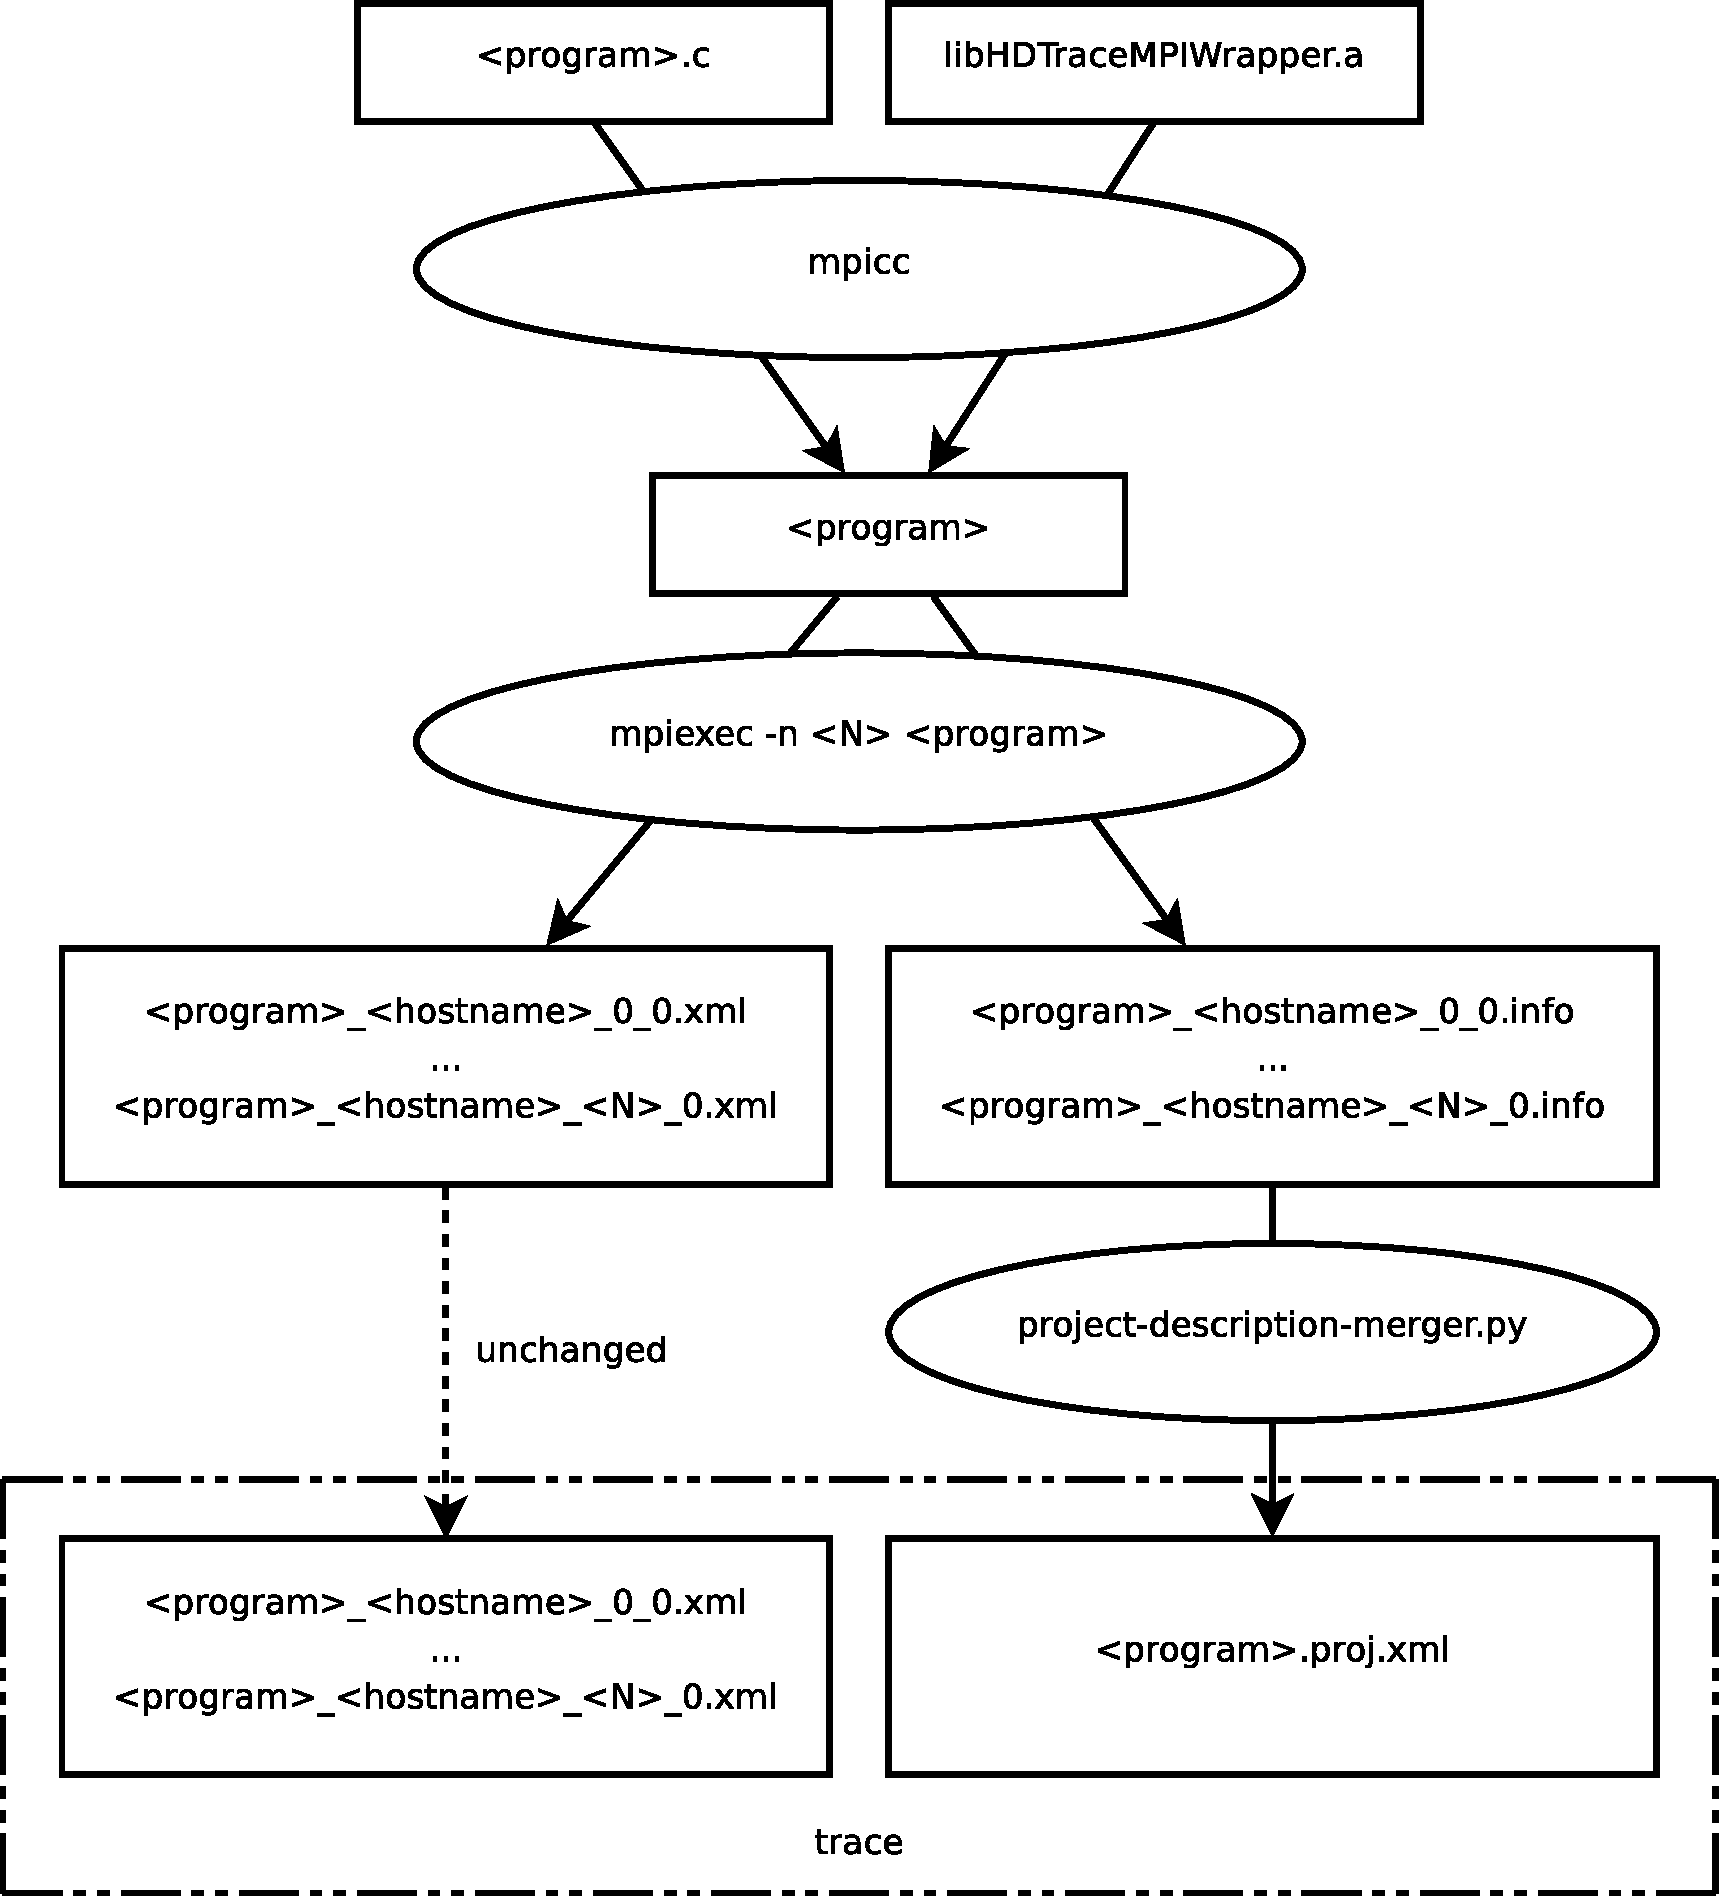
\includegraphics[width=0.6 \textwidth]{img/trace}
  \caption{Creating and processing a trace}
\end{figure}

\subsubsection{HDTraceWritingCLibrary}
The HDTraceWritingCLibrary is a component that has been split from the
MPI wrapper for better reusability. It offers an interface for writing
xml logs. It is possible to log xml tags including attributes and
elements, and it supports nesting of xml tags up to a certain
(defined) depth.

The main logging item is the \emph{state}, which is indicated by
\verb/hdT_logStateStart()/ and \verb/hdT_logStateEnd()/
\begin{lstlisting}
// trace is the structure that indicates the files to which data
// is being written. It is created by hdT_createTrace(...)
hdT_logStateStart(trace, "StateName");
// execution of the MPI calls, 
// logging of elements and attributes that belong to the state
hdT_logStateEnd(trace)
\end{lstlisting}

It also uses \verb/gettimeofday/ to log the time at which the state
has been started and finished.

There are two files that are created for each trace. One is the xml
file that holds data about the states that were logged. This file is
compatible with the logging format that is expected by other
tools. The second file is a plaintext (\verb/.info/) file that can be
used to store additional information.

\subsubsection{HDTraceMPIWrapper}
The mpi wrapper is the component that actually intercepts the MPI
calls and that determines which data is being logged. 

\subsubsection{Project Description Merger}
The script \verb/project-description-merger.py/ converts the trace of
a program into a form that is compliant with other PIOsim tools. More
precise, it uses data from the \verb/.info/-files to create a project
description xml file. The collection of xml files -- the xml trace files
created by all processes and the new description xml -- constitute a complete
trace. The \verb/.info/ files are then no longer needed.

\subsection{Design}
This section describes some decisions that were made
concerning the design of the MPI wrapper.

\subsubsection{Automatic code generation}
The wrapper functions that constitute the vital part of the MPI
wrapper are very similar in their structure. Because of that, they are
automatically generated by a script. This approach, while adding
another layer of complexity, greatly reduces possible mistakes that
would occur otherwise. The script obtains a list of functions from the
file \verb|interesting_funcs.h|. The connections -- which function
arguments are recorded with which attribute name -- are stored in the
file \verb|scripts/wrapper_conf.py|.

\subsubsection{Log format}
It is necessary that the output of the trace library must be
compatible with the tracing format that is used by the simulator,
HDJumpshot etc. This means a set of xml files that contain the MPI
function calls and their arguments, and one single project description
file that contains the information about the names of the other xml
files and miscellaneous information. The naming of the process files
must fulfill the naming convention
\begin{lstlisting}
<base name>_<level 1>_..._<level K>.trc
\end{lstlisting}
\verb/<base name>/ is the name of the project and \verb/<level 1>/
... \verb/<level K>/ constitute the representation of the file in a tree
structure.

The MPI wrapper uses the following topology and naming convention:
\begin{itemize}
\item \verb/<base name>/ is the name of the executable that is being
  traced. (It is extracted from \verb/*argv[0]/ of the arguments to
  \verb/MPI_Init()/
\item \verb/<level 1>/ is the hostname of the machine on which the
  process is running. It is obtained by a call to \verb/gethostname()/
\item \verb/<level 2>/ is the MPI rank of the
  process. (\verb/MPI_Comm_rank()/)
\item \verb/<level 3>/ is the number of the thread that belongs to the
  current process. The enumeration of threads depends on the order in
  which \verb/MPI_Init_thread()/ or \verb/MPI_Init/ is called and is
  usually arbitrary.
\end{itemize}

As discussed earlier, the project description file is not generated at
runtime because it would require communication between the
processes. Because we do not want to disrupt the program's original
MPI communication, the description file has to be created in a
postprocessing step. The postprocessing is done by the script
\verb/project-description-merger.py/. 

The project description file is an xml file with the root element
\verb/Application/. 

It contains the following sections: 
\begin{itemize}
\item \emph{FileList} This section contains the files that have been
  accessed by the program and their initial sizes. 
\begin{lstlisting}[caption=FileList section]
<FileList>
<File name="test.out">
 <InitialSize>16777216</InitialSize>
 <Distribution 
class="de.hd.pvs.piosim.model.inputOutput.distribution.SimpleStripe" />
 <ChunkSize>64K</ChunkSize>
</File>
</FileList>
\end{lstlisting}
The \verb/Distribution/ and \verb/ChukSize/ elements are not derived
from the trace file. They are relevant for the MPI simulator and can
be set by passing the corresponding command line arguments to the
merger script.
\item \emph{Topology} The topology section holds the information about
  the files that constitute the complete trace file. The \verb/Level/
  entries determine the names of the different levels. Those are fixed
  for program traces, with the values \emph{Hostname}, \emph{Rank},
  \emph{Thread}.

\begin{lstlisting}
 <Topology>
  <Level name="Hostname">
   <Level name="Rank">
    <Level name="Thread">
    </Level>
   </Level>
  </Level>
\end{lstlisting}

  The \emph{Label} section determines the names of the single xml
  trace files. If, for example, the Label section contains the
  following entries, the folder must also contain the files named
  \verb/<programname>_node01_0_0.trc/ and
  \verb/<programname>_node01_1_0.trc/.
\begin{lstlisting}
  <Label value="node01">
   <Label value="1">
    <Label value="0" />
   </Label>
   <Label value="0">
    <Label value="0" />
   </Label>
  </Label>
 </Topology>
\end{lstlisting}

\item \emph{CommunicatorList} This section lists all the communicators
  that are used in any traced call. The communicator's name, the
  participating ranks (\verb/global/, relative to
  \verb/MPI_COMM_WORLD/), the ID that this rank has relative to the
  new communicator (\verb/local/) and the ID that the communicator has
  in the tracefile (\verb/cid/).

  In the following example there are five ranks that each refer to the
  world communicator by the ID 0, and a second communicator where rank
  1 has the id one and rank 2 has the id 0. Rank 1 refers to the
  custom communicator by 1 and rank 2 by 2.
\begin{lstlisting}
<CommunicatorList>
  <Communicator name="WORLD">
   <Rank global="1" local="1" cid="0" />
   <Rank global="0" local="0" cid="0" />
   <Rank global="4" local="4" cid="0" />
   <Rank global="3" local="3" cid="0" />
   <Rank global="2" local="2" cid="0" />
  </Communicator>
  <Communicator name="">
   <Rank global="1" local="1" cid="1" />
   <Rank global="2" local="0" cid="2" />
  </Communicator>
\end{lstlisting}
\item \emph{Datatypes} The Datatypes section lists the datatypes that
  are used by each rank. In the following example, rank 1 uses the
  predefined, named datatype \verb/MPI_INT/ while rank 0 does not use
  any datatypes. The xml log of rank 1 refers to the datatype by the
  numerical id 1275069445.
\begin{lstlisting}
 <Datatypes>
  <Rank name="1" thread="0">
  <NAMED id="1275069445" name="MPI_INT"  />
  </Rank>
  <Rank name="0" thread="0">
  </Rank>
 </Datatypes>
\end{lstlisting}
  The name of the tag that represents a datatype is the name of the
  constant that is returned by \verb/MPI_Type_get_envelope/, without
  the \verb/MPI_/ prefix.

  The datatypes are stored per process, so it would have been
  reasonable to put this section into the individual xml traces. This
  has not been done because the xml traces should remain unchanged in
  the postprocessing step.
\end{itemize}

\subsubsection{Files}
An MPI function can access a file by using an MPI file handle, a file
name or both. An example for the first one would be
\verb/MPI_File_write/, \verb/MPI_File_delete/ for the second and
\verb/MPI_File_open/ for the last one.  Independent on the method we
need to log, which file is being accessed.  This is implemented by
assigning an id to each file that is used. When the file is opened via
\verb/MPI_File_open/ for the first time, the id is stored in one hash
map where the file name as the key and in a second map where the key
is the file handle. When the file is closed, the handle is removed
from the second hash map. On any consecutive openinig, the new file
handle can be associated with the original identifier via the file
name to id map.

The mapping and assigning of identifiers is carried out by the
functions
\begin{lstlisting}
static gint getFileId(MPI_File fh);
static gint getFileIdFromName(const char * name);
static gint getFileIdEx(MPI_File fh, const char * name);
\end{lstlisting}

Whenever a new identifier is assigned, these functions write the file
name, the id and the original size to the info file:
\begin{lstlisting}
File name="filetest_03.tmp" Size=0 id=2
\end{lstlisting}

In the xml trace, the file is refered to by the id (attribute \verb/file/) and the file name
on opening:
\begin{lstlisting}
<File_write_at_all_begin file='2' aid='0' 
      time='1240424724.531647' end='1240424724.531654' >
  <Data offset='0' size='1' count='1' type='1275068673' />
</File_write_at_all_begin>
\end{lstlisting}

\subsubsection{Time}
The hdTrace library sets a time stamp on the beginning and end of
every state. The time is obtained by \verb/gettimeofday/. It is
represented by the attributes \verb/time/ for the start of the state
and \verb/end/ for its end.
\begin{lstlisting}
<Init  time='1240424724.508182' end='1240424724.508183'  />
\end{lstlisting}

When the trace is run on different machines, the time must be properly
synchronised (via . 

\subsubsection{Data types}

MPI offers the possibility to create and use custom datatypes to
optimize access and transmission of complex structures. 
Datatypes are also used to set the visibility of certain parts of a
file.

Because of that it is necessary to identify data types and to log
their structure so access to a file can be reconstructed
correctly. The exact composition of a datatype is also needed for
performance analysis.

% how is an mpi datatype made
An MPI datatype can be created by a number of different functions that
take a different number of arguments. Fortunately, it offers a way of
reconstructing the call that was used to create a type: First,
\verb/MPI_Type_get_envelope/ has to be called to get the number of
arguments that were passed to the type-creating function, and the
\emph{combiner} that identifies the creating function. A second call
to \verb/MPI_Type_get_contents/ can be used to obtain the arguments
themselves. This mechanism is used to log the datatypes to the info
file.

Similar to other structures, MPI datatypes are assigned an identifier
on their first use by a logging routine. This happens by calling the
function \verb/getTypeId(MPI_Datatype type)/. \verb/getTypeId/ looks
up in a hashmap, if the datatype already has an identifier. If not, it
assigns a new id and calls \verb/writeTypeInfo(...)/ which writes the
creation arguments to the info file. If the datatype is a composet
datatype that consists of other datatypes, those are referenced while
writing the info file, which causes them to be logged as well. In the
end, all the information that is needed to reconstruct the datatype
will be recursively logged.

For example, creating a struct consisting of four \verb/MPI_INT/s and
five \verb/MPI_DOUBLE/s will produce the following output. 
\verb/id/ is the integer by which the datatype is refered to in the
log file. \verb/combiner/ is the name of the MPI constant that
identifies by which function the type has been
created. \verb/integers/, \verb/addresses/ and \verb/types/ are the
parameters that have been passed to that function. \verb/types/ uses
the trace-intern identifiers to refer to the types.
\begin{lstlisting}
Type id='1275069445' combiner='MPI_COMBINER_NAMED' name='MPI_INT'
Type id='1275070475' combiner='MPI_COMBINER_NAMED' name='MPI_DOUBLE'
Type id='-1946157050' combiner='MPI_COMBINER_STRUCT' name='' \
  integers='2;4;5;' addresses='6;7;' types='1275069445;1275070475;'
\end{lstlisting}

This is the code segment that would produce the above output.
\begin{lstlisting}
int blens[2] = {4, 5};
MPI_Aint inds[2] = {6, 7};
MPI_Datatype oldtypes[2] = {MPI_INT, MPI_DOUBLE};
MPI_Type_struct(2, blens, inds, oldtypes, &type6);
// use type6 in a transmission that is logged
\end{lstlisting}

\subsubsection{Communicators}
There are two main issues with communicators: We need to know who is
participating in a transmission, and the translation between global
ranks to the ranks that are assigned relative to the communicator.

The logging takes place in a straightforward fashion: Every
communicator gets an identifier on the first access and this
identifier and the translation map is written to the info file.
The name of the communicator is also written, albeit it is rarely
useful in cases other than the world and the self communicators.

In the following example the program used three communicators, the
world communicator, one communicator with the global ranks 1 and 2 and
one with the global ranks 1 and three.
\begin{lstlisting}
Comm map='0->0;1->1;2->2;3->3;4->4;' id=0 name='WORLD'
Comm map='1->1;2->0;' id=1 name=''
Comm map='1->1;3->0;' id=2 name=''
\end{lstlisting}

\subsubsection{Non-blocking communication}

There are two types of non-blocking communication provided by MPI.
\begin{itemize}
\item \verb/MPI_I/ non-blocking function calls that return an
  \verb/MPI_Request/ structure that can be used to query the state of
  the call.
\item Collective I/O operations can be performed using a split
  collective call. This means that the function,
  e.g. \verb/MPI_File_read_all/ is split into
  \verb/MPI_File_read_all_begin/ and \verb/MPI_File_read_all_end/.
  Only one split collective call may be active for each file.
\end{itemize}

Because of semantic similarities between the two mechanisms they share
the logging representation. Similar to the logging of files,
communicators and datatypes, each \verb/MPI_Request/ is assigned an id
by which it is refered to when logging related calls. 

The first version is logged like this:
\begin{lstlisting}
<Isend size='1' count='1' type='1275068673' toRank='1' toTag='0' \
  cid='0' rid='1'\  time='1240497420.078912' end='1240497420.078981'  />
<Isend size='1' count='1' type='1275068673' toRank='2' toTag='0' \
  cid='0' rid='2'  time='1240497420.078987' end='1240497420.079006'  />
<Wait  time='1240497420.079011' end='1240497420.079028' >
  <For rid='1' />
</Wait>
<Wait  time='1240497420.079034' end='1240497420.079037' >
  <For rid='2' />
</Wait>
\end{lstlisting}
Here, two non-blocking \verb/Isend/s are issued with the request
identifiers (\verb/rid/) 1 and 2. Then the program watis for the first
and second sending to complete.

The split collective calls are also assigned an \verb/rid/, which is
bound to the file handle. This works because each file may have at
most one open split collective call. The \verb/_end/ part of the call
is then logged exactly like a \verb/Wait/.

This is, for example, how a \verb/MPI_File_write_at_all_begin/ -
\verb/MPI_File_write_at_all_end/ pair is logged:

\begin{lstlisting}
<File_write_at_all_begin fid='0' rid='0'  time='1240497420.073870' end='1240497420.076409' >
  <Data offset='0' size='1' count='1' type='1275068673' />
</File_write_at_all_begin>
<Wait  time='1240497420.076415' end='1240497420.076418' >
  <For rid='0' />
</Wait>
\end{lstlisting}

\subsubsection{Threading}

The wrapper has been programmed with threading in mind. The TLS
(thread local storage) mechanism of the gcc compiler is used to ensure
that global variables are limited to the current thread. Also,
\verb/MPI_Init/ (or \verb/MPI_Init_thread/) are using a counter to
keep track, how often they have been called. This is used to give each
thread a separate tracefile. The thread number is the last number in
the log file names.

It must be noted that thread support has not been carefully
tested. Also, the project description merger handles trace files from
different ranks and trace files from different threads in the same
way. 

\section{Environment variables and command line options} 
\subsection{HDTraceMPIWrapper.a}
The behaviour of the tracing library can be adjusted by setting
certain environment variables before running a program. For example,
you can force flushing the write buffer on each write by setting
{\verb HDTRACE_FORCE_FLUSH }:
\begin{lstlisting}
HDTRACE_FORCE_FLUSH=1 ./mpi-io-test
\end{lstlisting}

The following variables are supported:

\subsubsection{HDTRACE\_FORCE\_FLUSH}
{\verb HDTRACE_FORCE_FLUSH=0 } means, the wrapper flushes the write
buffer on its own discretion, usually only when the buffer is full or
the file is closed. This is the default.

{\verb HDTRACE_FORCE_FLUSH=1 } causes the wrapper to flush the
write buffer on every write.


\subsubsection{HDTRACE\_NESTED}
This variable influences, whever nested function calls should be
traced. A nested call is a call to an MPI routine from within an MPI
routine.

{\verb HDTRACE_NESTED=0 } Only the outer function call is being logged.

{\verb HDTRACE_NESTED=1 } Nested calls up to a certain depth are
logged. The depth is determined by the constant {\verb
  HD_LOG_MAX_DEPTH }, defined in {\verb hdTrace.h }

\subsubsection{HDTRACE\_FILE\_INFO}
This variable determines, if the MPI\_Info structure that is given
to {\verb MPI_File_delete }, {\verb MPI_File_set_view }, {\verb
  MPI_File_set_info } or {\verb MPI_File_open } should be logged.   

{\verb HDTRACE_FILE_INFO=0 } The file information is not logged

{\verb HDTRACE_FILE_INFO=1 } The file information is logged

\subsubsection{HDTRACE\_ALL\_FUNCTIONS}
This variable determines, if ordinary functions should be logged. An
ordinary function is one that appears in {\verb
  include/interesting_funcs.h } but does not have any elements or
attributes other than start and end time being logged.

{\verb HDTRACE_ALL_FUNCTIONS=0 } ordinary functions are not logged.

{\verb HDTRACE_ALL_FUNCTIONS=1 } ordinary functions are logged. This
is the default.

\subsection{project-description-merger.py}

The project description merger creates a single xml file from the
collection of info files that have been written by the different MPI
processes. 

\subsubsection{Usage}
\begin{lstlisting}
project-description-merger.py -o <outfile.trc> [-d <description>] \
[--distribution-class=<class>] \
[--chunk-size=<size>] \
<log1>.info <log2>.info ... <logN>.info
\end{lstlisting}

\verb -o  \verb <outfile>  (required): The output file. The naming conventions for the
trace files are { \verb <program-name>_<hostname>_<rank>_<thread>.trc }. 

 It is advised to use { \verb <program-name>.trc } as output
 filename. This is expected by other PIOsim applications.

{ \verb -d  \verb <description> } (optional): The description of the
project. This can be anything. 

\section{Future Work}

\subsection{Thread safety}
The wrapper has been programmed for being usable with multithreaded
MPI applications. However, this has not yet been excessively tested.

\subsection{File name ambiguity}
If the same file is accessed using different names it will appear in
the log as two different files. Using a \lstinline{realpath()}-like
function is advisable. Unfortunately, \lstinline{realpath()} does not
handle pvfs filenames

\subsection{Packaging}
Currently, the necessary MPI headers are copied into the project's
include directory. This should be handled by the configuration script.

\appendix

\section{Logged attributes and elements}

This section lists the format of the xml log file. Each xml tag has
the name of the logged function without \verb/MPI_/ prefix. 
The type of the values is given in printf-compatible notation.

\subsection{Common attributes}

\begin{itemize}
\item[size] An approximation of the size of the data that is accessed,
  in bytes. It is calculated by taking the product of the element
  count and the type size as returned by \verb/MPI_Type_size/.
\item[cid] The id of the communicator that is used
\item[type] The id of the type that is used.
\item[time] The time at which the MPI function is called.
\item[end] The time at which the MPI function returned.
\item[fid] The id of the file that is referenced.
\item[rid] The id of the request that is used.
\end{itemize}

\subsection{List of logged attributes}


\subsection{MPI\_Allgather}
\begin{lstlisting}
<Allgather size='%lld' recvSize='%lld' cid='%d' count='%d' tid='%d' recvCount='%d' recvtid='%d' time='%f' end='%f' />
\end{lstlisting}

\subsection{MPI\_Allgatherv}
\begin{lstlisting}
<Allgatherv size='%lld' cid='%d' count='%d' tid='%d' time='%f' end='%f' />
\end{lstlisting}

\subsection{MPI\_Allreduce}
\begin{lstlisting}
<Allreduce size='%lld' cid='%d' count='%d' tid='%d' time='%f' end='%f' />
\end{lstlisting}

\subsection{MPI\_Alltoall}
\begin{lstlisting}
<Alltoall size='%lld' cid='%d' count='%d' tid='%d' time='%f' end='%f' />
\end{lstlisting}

\subsection{MPI\_Alltoallv}
\begin{lstlisting}
<Alltoallv cid='%d' time='%f' end='%f' />
\end{lstlisting}

\subsection{MPI\_Barrier}
\begin{lstlisting}
<Barrier cid='%d' time='%f' end='%f' />
\end{lstlisting}

\subsection{MPI\_Bcast}
\begin{lstlisting}
<Bcast size='%lld' rootRank='%d' cid='%d' count='%d' tid='%d' time='%f' end='%f' />
\end{lstlisting}

\subsection{MPI\_Bsend}
\begin{lstlisting}
<Bsend size='%lld' count='%d' tid='%d' toRank='%d' toTag='%d' cid='%d' time='%f' end='%f' />
\end{lstlisting}

\subsection{MPI\_Exscan}
\begin{lstlisting}
<Exscan size='%lld' cid='%d' count='%d' tid='%d' time='%f' end='%f' />
\end{lstlisting}

\subsection{MPI\_File\_close}
\begin{lstlisting}
<File_close fid='%d' time='%f' end='%f' />
\end{lstlisting}

\subsection{MPI\_File\_delete}
\begin{lstlisting}
<File_delete fid='%d' time='%f' end='%f' />
\end{lstlisting}

\subsection{MPI\_File\_get\_size}
\begin{lstlisting}
<File_get_size fid='%d' size='%lld' time='%f' end='%f' />
\end{lstlisting}

\subsection{MPI\_File\_iread}
\begin{lstlisting}
<File_iread fid='%d' rid='%d' offset='%lld' size='%lld' count='%d' tid='%d' time='%f' end='%f' />
\end{lstlisting}

\subsection{MPI\_File\_iread\_at}
\begin{lstlisting}
<File_iread_at fid='%d' rid='%d' offset='%lld' size='%lld' count='%d' tid='%d' time='%f' end='%f' />
\end{lstlisting}

\subsection{MPI\_File\_iread\_shared}
\begin{lstlisting}
<File_iread_shared fid='%d' rid='%d' time='%f' end='%f' />
\end{lstlisting}

\subsection{MPI\_File\_iwrite}
\begin{lstlisting}
<File_iwrite fid='%d' rid='%d' offset='%lld' size='%lld' count='%d' tid='%d' time='%f' end='%f' />
\end{lstlisting}

\subsection{MPI\_File\_iwrite\_at}
\begin{lstlisting}
<File_iwrite_at fid='%d' rid='%d' offset='%lld' size='%lld' count='%d' tid='%d' time='%f' end='%f' />
\end{lstlisting}

\subsection{MPI\_File\_iwrite\_shared}
\begin{lstlisting}
<File_iwrite_shared fid='%d' rid='%d' time='%f' end='%f' />
\end{lstlisting}

\subsection{MPI\_File\_open}
\begin{lstlisting}
<File_open cid='%d' name='%s' flags='%d' fid='%d' time='%f' end='%f' />
\end{lstlisting}

\subsection{MPI\_File\_preallocate}
\begin{lstlisting}
<File_preallocate fid='%d' size='%lld' time='%f' end='%f' />
\end{lstlisting}

\subsection{MPI\_File\_read}
\begin{lstlisting}
<File_read fid='%d' offset='%lld' size='%lld' count='%d' tid='%d' time='%f' end='%f' />
\end{lstlisting}

\subsection{MPI\_File\_read\_all}
\begin{lstlisting}
<File_read_all fid='%d' offset='%lld' size='%lld' count='%d' tid='%d' time='%f' end='%f' />
\end{lstlisting}

\subsection{MPI\_File\_read\_all\_begin}
\begin{lstlisting}
<File_read_all_begin fid='%d' rid='%d' time='%f' end='%f' />
\end{lstlisting}

\subsection{MPI\_File\_read\_all\_end}
\begin{lstlisting}
<File_read_all_end  time='%f' end='%f' />
\end{lstlisting}

\subsection{MPI\_File\_read\_at}
\begin{lstlisting}
<File_read_at fid='%d' offset='%lld' size='%lld' count='%d' tid='%d' time='%f' end='%f' />
\end{lstlisting}

\subsection{MPI\_File\_read\_at\_all}
\begin{lstlisting}
<File_read_at_all fid='%d' offset='%lld' size='%lld' count='%d' tid='%d' time='%f' end='%f' />
\end{lstlisting}

\subsection{MPI\_File\_read\_at\_all\_begin}
\begin{lstlisting}
<File_read_at_all_begin fid='%d' rid='%d' offset='%lld' size='%lld' count='%d' tid='%d' time='%f' end='%f' />
\end{lstlisting}

\subsection{MPI\_File\_read\_at\_all\_end}
\begin{lstlisting}
<File_read_at_all_end  time='%f' end='%f' />
\end{lstlisting}

\subsection{MPI\_File\_read\_ordered}
\begin{lstlisting}
<File_read_ordered fid='%d' size='%lld' count='%d' tid='%d' time='%f' end='%f' />
\end{lstlisting}

\subsection{MPI\_File\_read\_ordered\_begin}
\begin{lstlisting}
<File_read_ordered_begin fid='%d' rid='%d' time='%f' end='%f' />
\end{lstlisting}

\subsection{MPI\_File\_read\_ordered\_end}
\begin{lstlisting}
<File_read_ordered_end  time='%f' end='%f' />
\end{lstlisting}

\subsection{MPI\_File\_read\_shared}
\begin{lstlisting}
<File_read_shared fid='%d' size='%lld' count='%d' tid='%d' time='%f' end='%f' />
\end{lstlisting}

\subsection{MPI\_File\_seek}
\begin{lstlisting}
<File_seek fid='%d' relative-offset='%lld' whence='%s' offset='%lld' time='%f' end='%f' />
\end{lstlisting}

\subsection{MPI\_File\_seek\_shared}
\begin{lstlisting}
<File_seek_shared fid='%d' relative-offset='%lld' whence='%s' offset='%lld' time='%f' end='%f' />
\end{lstlisting}

\subsection{MPI\_File\_set\_atomicity}
\begin{lstlisting}
<File_set_atomicity fid='%d' flag='%d' time='%f' end='%f' />
\end{lstlisting}

\subsection{MPI\_File\_set\_info}
\begin{lstlisting}
<File_set_info fid='%d' time='%f' end='%f' />
\end{lstlisting}

\subsection{MPI\_File\_set\_size}
\begin{lstlisting}
<File_set_size fid='%d' size='%lld' time='%f' end='%f' />
\end{lstlisting}

\subsection{MPI\_File\_set\_view}
\begin{lstlisting}
<File_set_view fid='%d' offset='%lld' etid='%d' filetid='%d' representation='%s' time='%f' end='%f' />
\end{lstlisting}

\subsection{MPI\_File\_sync}
\begin{lstlisting}
<File_sync fid='%d' time='%f' end='%f' />
\end{lstlisting}

\subsection{MPI\_File\_write}
\begin{lstlisting}
<File_write fid='%d' offset='%lld' size='%lld' count='%d' tid='%d' time='%f' end='%f' />
\end{lstlisting}

\subsection{MPI\_File\_write\_all}
\begin{lstlisting}
<File_write_all fid='%d' offset='%lld' size='%lld' count='%d' tid='%d' time='%f' end='%f' />
\end{lstlisting}

\subsection{MPI\_File\_write\_all\_begin}
\begin{lstlisting}
<File_write_all_begin fid='%d' rid='%d' time='%f' end='%f' />
\end{lstlisting}

\subsection{MPI\_File\_write\_all\_end}
\begin{lstlisting}
<File_write_all_end  time='%f' end='%f' />
\end{lstlisting}

\subsection{MPI\_File\_write\_at}
\begin{lstlisting}
<File_write_at fid='%d' offset='%lld' size='%lld' count='%d' tid='%d' time='%f' end='%f' />
\end{lstlisting}

\subsection{MPI\_File\_write\_at\_all}
\begin{lstlisting}
<File_write_at_all fid='%d' offset='%lld' size='%lld' count='%d' tid='%d' time='%f' end='%f' />
\end{lstlisting}

\subsection{MPI\_File\_write\_at\_all\_begin}
\begin{lstlisting}
<File_write_at_all_begin fid='%d' rid='%d' time='%f' end='%f' />
\end{lstlisting}

\subsection{MPI\_File\_write\_at\_all\_end}
\begin{lstlisting}
<File_write_at_all_end  time='%f' end='%f' />
\end{lstlisting}

\subsection{MPI\_File\_write\_ordered}
\begin{lstlisting}
<File_write_ordered fid='%d' size='%lld' count='%d' tid='%d'  time='%f' end='%f' />
\end{lstlisting}

\subsection{MPI\_File\_write\_ordered\_begin}
\begin{lstlisting}
<File_write_ordered_begin fid='%d' rid='%d' time='%f' end='%f' />
\end{lstlisting}

\subsection{MPI\_File\_write\_ordered\_end}
\begin{lstlisting}
<File_write_ordered_end  time='%f' end='%f' />
\end{lstlisting}

\subsection{MPI\_File\_write\_shared}
\begin{lstlisting}
<File_write_shared fid='%d' size='%lld' count='%d' tid='%d' time='%f' end='%f' />
\end{lstlisting}

\subsection{MPI\_Gather}
\begin{lstlisting}
<Gather size='%lld' recvSize='%lld' root='%d' cid='%d' count='%d' tid='%d' recvCount='%d' recvtid='%d' time='%f' end='%f' />
\end{lstlisting}

\subsection{MPI\_Gatherv}
\begin{lstlisting}
<Gatherv size='%lld' root='%d' cid='%d' count='%d' tid='%d' time='%f' end='%f' />
\end{lstlisting}

\subsection{MPI\_Ibsend}
\begin{lstlisting}
<Ibsend size='%lld' count='%d' tid='%d' toRank='%d' toTag='%d' cid='%d' rid='%d' time='%f' end='%f' />
\end{lstlisting}

\subsection{MPI\_Iprobe}
\begin{lstlisting}
<Iprobe source='%d' tag='%d' cid='%d' time='%f' end='%f' />
\end{lstlisting}

\subsection{MPI\_Irecv}
\begin{lstlisting}
<Irecv fromRank='%d' fromTag='%d' cid='%d' rid='%d' time='%f' end='%f' />
\end{lstlisting}

\subsection{MPI\_Irsend}
\begin{lstlisting}
<Irsend size='%lld' count='%d' tid='%d' toRank='%d' toTag='%d' cid='%d' rid='%d' time='%f' end='%f' />
\end{lstlisting}

\subsection{MPI\_Isend}
\begin{lstlisting}
<Isend size='%lld' count='%d' tid='%d' toRank='%d' toTag='%d' cid='%d' rid='%d' time='%f' end='%f' />
\end{lstlisting}

\subsection{MPI\_Issend}
\begin{lstlisting}
<Issend size='%lld' count='%d' tid='%d' toRank='%d' toTag='%d' cid='%d' rid='%d' time='%f' end='%f' />
\end{lstlisting}

\subsection{MPI\_Recv}
\begin{lstlisting}
<Recv fromRank='%d' fromTag='%d' cid='%d' time='%f' end='%f' />
\end{lstlisting}

\subsection{MPI\_Reduce}
\begin{lstlisting}
<Reduce size='%lld' rootRank='%d' cid='%d' count='%d' tid='%d' time='%f' end='%f' />
\end{lstlisting}

\subsection{MPI\_Reduce\_scatter}
\begin{lstlisting}
<Reduce_scatter cid='%d' time='%f' end='%f' />
\end{lstlisting}

\subsection{MPI\_Rsend}
\begin{lstlisting}
<Rsend size='%lld' count='%d' tid='%d' toRank='%d' toTag='%d' cid='%d' time='%f' end='%f' />
\end{lstlisting}

\subsection{MPI\_Scan}
\begin{lstlisting}
<Scan size='%lld' cid='%d' count='%d' tid='%d' time='%f' end='%f' />
\end{lstlisting}

\subsection{MPI\_Scatter}
\begin{lstlisting}
<Scatter size='%lld' recvSize='%lld' root='%d' cid='%d' count='%d' tid='%d' recvCount'%d' recvtid='%d' time='%f' end='%f' />
\end{lstlisting}

\subsection{MPI\_Scatterv}
\begin{lstlisting}
<Scatterv recvSize='%lld' root='%d' cid='%d' recvCount='%d' recvtid='%d' time='%f' end='%f' />
\end{lstlisting}

\subsection{MPI\_Send}
\begin{lstlisting}
<Send size='%lld' count='%d' tid='%d' toRank='%d' toTag='%d' cid='%d' time='%f' end='%f' />
\end{lstlisting}

\subsection{MPI\_Sendrecv}
\begin{lstlisting}
<Sendrecv size='%lld' toRank='%d' toTag='%d' fromRank='%d' fromTag='%d' cid='%d' count='%d' tid='%d' time='%f' end='%f' />
\end{lstlisting}

\subsection{MPI\_Sendrecv\_replace}
\begin{lstlisting}
<Sendrecv_replace sendSize='%lld' toRank='%d' toTag='%d' fromRank='%d' fromTag='%d' cid='%d' count='%d' tid='%d' time='%f' end='%f' />
\end{lstlisting}

\subsection{MPI\_Ssend}
\begin{lstlisting}
<Ssend size='%lld' count='%d' tid='%d' toRank='%d' toTag='%d' cid='%d' time='%f' end='%f' />
\end{lstlisting}

\subsection{MPI\_Type\_commit}
\begin{lstlisting}
<Type_commit tid='%d' time='%f' end='%f' />
\end{lstlisting}

\subsection{MPI\_Type\_vector}
\begin{lstlisting}
<Type_vector oldTid='%d' time='%f' end='%f' />
\end{lstlisting}

\subsection{MPI\_hdT\_Test\_nested}
\begin{lstlisting}
<hdT_Test_nested depth='%d' time='%f' end='%f' />
\end{lstlisting}

\section{Datatype representation in the project description}

\subsection{MPI\_COMBINER\_DUP}
\begin{lstlisting}
<DUP id="%d" name="%s" oldType="%d" />
\end{lstlisting}

\subsection{MPI\_COMBINER\_CONTIGUOUS}
\begin{lstlisting}
<CONTIGUOUS id="%d" name="%s" count="%d" oldType="%d" />
\end{lstlisting}

\subsection{MPI\_COMBINER\_VECTOR}

\begin{lstlisting}
<VECTOR id="%d" name="%s" count="%d" blocklength="%d" stride="%d" oldType="%d" />
\end{lstlisting}

\subsection{MPI\_COMBINER\_HVECTOR, MPI\_COMBINER\_HVECTOR\_INTEGER}
\begin{lstlisting}
<HVECTOR id="%d" name="%s" count="%d" blocklength="%d" stride="%d" oldType="%d" /> 
<HVECTOR_INTEGER id="%d" name="%s" count="%d" blocklength="%d" stride="%d" oldType="%d" /> 
\end{lstlisting}

\subsection{MPI\_COMBINER\_RESIZED}

\begin{lstlisting}
<RESIZED id="%d" name="%s" lowerBound="%d" extend="%d" oldType="%d" />
\end{lstlisting}

\subsection{MPI\_COMBINER\_INDEXED}
\begin{lstlisting}
<INDEXED id="%d" name="%s" count="%d" oldType="%d" >
  <BLOCK len="%d" index="%d />
  <BLOCK len="%d" index="%d />
  ...
</INDEXED>
\end{lstlisting}

\subsection{MPI\_COMBINER\_HINDEXED}
\begin{lstlisting}
<HINDEXED id="%d" name="%s" count="%d" oldType="%d" >
  <BLOCK len="%d" index="%d />
  <BLOCK len="%d" index="%d />
  ...
</HINDEXED>
\end{lstlisting}

\subsection{MPI\_COMBINER\_INDEXED\_BLOCK}
\begin{lstlisting}
<INDEXED_BLOCK id="%d" name="%s" count="%d" oldType="%d" blockLength="%d">
  <Block displacement="%s" />
  <Block displacement="%s" />
  ...
</HINDEXED_BLOCK>
\end{lstlisting}

\subsection{MPI\_COMBINER\_STRUCT}
\begin{lstlisting}
<STRUCT id="%d" name="%s" count="%d" >
  <Type id="%s" displacement="%s" blocklen="%s"/>
</STRUCT>
\end{lstlisting}

\subsection{MPI\_COMBINER\_STRUCT\_INTEGER}
\begin{lstlisting}
<STRUCT_INTEGER id="%d" name="%s" count="%d" >
  <Type id="%s" displacement="%s" blocklen="%s"/>
</STRUCT_INTEGER>
\end{lstlisting}

\subsection{MPI\_COMBINER\_SUBARRAY}
\begin{lstlisting}
<SUBARRAY id="%d" name="%s" count="%d" order="%s">
  <Dimension size="%s" subsize="%s" start="%s" />
  <Dimension size="%s" subsize="%s" start="%s" />
  ...
</SUBARRAY>
\end{lstlisting}
The attribute \lstinline{order} is either \lstinline{MPI_ORDER_C} or
\lstinline{MPI_ORDER_FORTRAN}. 

\subsection{MPI\_COMBINER\_DARRAY}
\begin{lstlisting}
<DARRAY id="%d" name="%s" size="%d" order="%s" rank="%d" dims="%d">
  <Dimension gsize="%d" distrib="%s" darg="%d" psize="%d" />
  <Dimension gsize="%d" distrib="%s" darg="%d" psize="%d" />
  ...
</DARRAY>
\end{lstlisting}
The attribute \lstinline{order} is either \lstinline{MPI_ORDER_C} or
\lstinline{MPI_ORDER_FORTRAN}.

The attribute \lstinline{distrib} has one of the values 
\begin{lstlisting}
MPI_DISTRIBUTE_BLOCK
MPI_DISTRIBUTE_CYCLIC
MPI_DISTRIBUTE_NONE
MPI_DISTRIBUTE_DFLT_DARG
\end{lstlisting}

\bibliography{references}
\bibliographystyle{alpha}

\end{document}
